\documentclass[11pt,a4paper]{report}
\usepackage[utf8]{inputenc}
\usepackage[french]{babel}
\usepackage[T1]{fontenc}
\usepackage{amsmath}
\usepackage{amsfonts}
\usepackage{amssymb}
\usepackage{xcolor}
\usepackage{gensymb}

\usepackage{geometry}
\geometry{hmargin=2.5cm,vmargin=1.5cm}
\usepackage{wasysym}
\usepackage{graphicx}

\author{Mathieu Sarrat}
\title{LP8 - Phénomènes de Transport}

\makeatletter
\renewcommand{\thesection}{\@arabic\c@section}
\makeatother


\begin{document}
\maketitle
\newpage
\section*{Pré-requis, objectifs, recommandations}

\subsubsection*{Niveau :}
\begin{itemize}
	\item Licence de physique
\end{itemize}

\subsubsection*{Pré-requis :}
\begin{itemize}
	\item Cours de thermodynamique
	\item Cours de mécanique des fluides
	\item Conduction électrique 
\end{itemize}

\subsubsection*{Matériel :}
\begin{itemize}
	\item 2 béchers d'eau, une cartouche d'encre et un compas pour la percer,
	\item une casserole ou une plaque métallique, une plaque en bois, deux glaçons.
\end{itemize}

\section*{Introduction}
Jusqu'à présent nous avons considéré des systèmes à l'état d'équilibre thermodynamique et des transformations reliant deux états d'équilibre. Lorsqu'un système est en équilibre thermodynamique :
\begin{itemize}
\item les grandeurs intensives le caractérisant (pression, température, potentiel chimique, aimantation etc...) sont stationnaires (invariantes dans le temps) et homogènes (sans dépendance spatiale), ce qui se traduit par l'absence de flux de matière et d'énergie à l'intérieur du système;
\item cela implique que ces mêmes grandeurs sont égales à celles du milieu extérieur à la frontière du système : égalité de la température, de la pression et du potentiel chimique (équilibre thermique, équilibre mécanique et équilibre chimique/osmotique simultanés). Une transformation n'aura lieu que si les variables décrivant le milieu extérieur changent, par exemple sous l'effet d'un opérateur.\\
\end{itemize}

Que se passe-t-il lorsque le système comporte des inhomogénéités ?\\ 

Commençons par un exemple pratique : si on verse une goutte d'encre dans un verre d'eau, on introduit une inhomogénéité de concentration en encre dans l'eau. On constante que l'encre se répand progressivement dans l'eau. Au bout d'un certain temps, la concentration en encre s'homogénéise. Si on utilise une cuillère pour mélanger, l'homogénéisation se fait bien plus rapidement. Dans les deux cas, on dit qu'il y a eu transport de matière, des régions de forte concentration vers les régions de faible concentration. Dans le premier cas, il n'y a pas eu de déplacement d'eau. Dans le second cas, si.\\ 

Lorsqu'on met en contact deux objets de températures différentes et qu'on attend suffisamment longtemps, la température finit par s'homogénéiser. Il y a eu transport d'énergie sous forme de chaleur, depuis le système le plus chaud vers le système le plus froid.\\

\newpage
\section{Principe d'une description générale macroscopique}

Dans la vie de tous les jours, les systèmes homogènes sont rares. Pour autant, nous sommes capables de mesurer la température de l'air ou la pression atmosphérique en un point donné, quand bien même l'ensemble de l'atmosphère n'est pas à l'équilibre thermodynamique. Quelles sont les conditions pour que ces mesures aient du sens ? Ou plutôt, peut-on utiliser des notions de thermodynamique même lorsqu'un système est inhomogène ?

\subsection{Équilibre thermodynamique local}

	Les notions fort convenables de pression, de température ou de masse volumique sont en réalité 		des moyennes de grandeurs microscopiques, calculées en considérant la matière comme constituée 		de particules. Ces moyennes n'ont de sens que sur un volume élémentaire représentatif 
	$d\mathcal{V}$, de longueur caractéristique $L$.\\ 
	
	\textbf{Élémentaire}, car ce volume doit être de petite taille par rapport à la taille du 			système et par rapport à la taille des variations, des tendances, de grande échelle :
	\begin{equation}
		L << L_c, L_g
	\end{equation}		
	où $L_c$ désigne la taille du système et $L_g$ la longueur caractéristique des gradients 			macroscopiques.\\
	
	\textbf{Représentatif} car il doit être suffisamment grand pour que l'on puisse moyenner les 		grandeurs microscopiques et faire disparaître leurs variations liées au caractère « granuleux » 	du milieu. Pour cela, il faut
	\begin{equation}
		L >> d, \ell
	\end{equation}
	où $\ell$ désigne le libre parcours moyen et $d$ la distance moyenne entre deux particules. 		Les collisions interviennent dans cette définition car elles participent à la relaxation des 		gradients.\\
	 
	Cette échelle de longueur, ni trop petite, ni trop grande, pour laquelle le système est 			localement homogène, mais permettant de tenir compte de profils de grandeurs physiques 				suffisamment doux, est qualifiée de \textbf{mésoscopique}.\\
	
	Si cette échelle mésoscopique existe, il est possible de définir un équilibre thermodynamique 		local et alors on peut découper le système en volumes mésoscopiques pouvant être considérés 		comme des systèmes à l'équilibre thermodynamique. On pourra utiliser localement les notions de 		température, de pression, de masse volumique, et ces quantités pourront présenter des gradients 	à grande échelle dans le système. Choisissons un $d\mathcal{V}$ centré autour du point 
	$\bold{r}$. On peut alors définir à tout instant $t$ un équilibre thermodynamique local autour 		de $\bold{r}$, et définir une température en ce point $T(\bold{r})$, un champ des vitesses si 		le milieu est déformable $\bold{v}(\bold{r})$, une pression $p(\bold{r})$, une masse 				volumique $\rho(\bold{r})$ etc ...\\
	
	Chaque élément de volume $d\mathcal{V}$ n'étant pas à l'équilibre avec ses voisins du fait des 		gradients, il en résulte l'existence d'échanges de matière ou d'énergie entre ces éléments de 		volume. Ce sont des transformations internes au système qui vont donner lieu aux phénomènes de 		transport dont nous allons parler. Ces transformations justifient la réintroduction du temps 
	$t$ comme dépendance des variables intensives ($T(\bold{r},t)$, $p(\bold{r},t)$, 
	$\rho(\bold{r},t)$).\\ 
	
	Dans ce cas, les grandeurs physiques moyennées sur $d\mathcal{V}$ comme la température, la 			pression, le champ des vitesses ou encore la densité volumique de particules ont un réel sens 		d'un point de vue statistique : elles sont représentatives de l'état des particules contenues 		dans le volume car il y a suffisamment de vraies particules dans $d\mathcal{V}$ et car la 			distribution statistique des grandeurs microscopiques est voisine d'une gaussienne (grâce aux 		collisions).\\
	
	\subsubsection*{Remarque}
	Dans un état d'équilibre thermodynamique, $d\mathcal{V}$ correspond en fait au volume de tout 		le système, ce dernier étant homogène à l'échelle mésoscopique et à l'échelle macroscopique.
	
	\subsubsection*{Méthode générale}
	Pour décrire un phénomène de transport de façon macroscopique, nous allons procéder avec la 		méthode générale suivante :
	\begin{itemize}
	\item \textcolor{red}{Etape 1 :} faire un bilan de la quantité transportée pour obtenir une 			équation de conservation (masse, charge, énergie interne, quantité de mouvement),
	\item \textcolor{red}{Etape 2 :} modéliser les flux de matière et d'énergie,
	\item \textcolor{red}{Etape 3 :} combiner ces deux points.
	\end{itemize}

\subsection{Bilan d'une grandeur extensive}

\subsubsection{Grandeur extensive X}
Soit X une grandeur extensive quelconque, dans un système de volume $V$ \textbf{délimité par une surface fixe de contrôle} S. En raison de l'équilibre thermodynamique local, la quantité de X contenue dans $d\mathcal{V}$ s'écrit
\begin{equation}
	dX = x_v(\bold{r},t)d\mathcal{V}, \quad\text{où }x_v\;\text{désigne la densité volumique de X}.
\end{equation}
Pour le système complet,
\begin{equation}
	X = \iiint x_v(\bold{r},t) d\mathcal{V}.
\end{equation}
Exemples : charge électrique, masse, quantité de mouvement \textcolor{red}{(écrire au tableau)}.

\subsubsection{Bilan de X}
Soit un système de volume $V$. Entre $t_1 = t$ et $t_2 = t + dt$, où $dt$ est infinitésimal, X varie de dX :
La surface de contrôle S étant fixe, $V(t+dt) = V(t)$ et
\begin{equation}
	dX = X(t+dt) - X(t) 
	= \iiint x_v(\bold{r},t+dt) d\mathcal{V} - \iiint x_v(\bold{r},t) d\mathcal{V}
	= dt \iiint \frac{\partial x_v}{\partial t} d\mathcal{V}.\\
\end{equation}

Par ailleurs, on peut écrire
\begin{equation}	
	\boxed{dX = \delta X^r + \delta X^c},
\end{equation}
où $\delta X^r$ est la quantité échangée avec le milieu extérieur et $\delta X^c$ la quantité créée (ou détruite) dans le système. Ces quantités sont positives si le milieu reçoit/créée, négatives s'il donne/détruit.

\begin{figure}[h!]
	\begin{center}
  		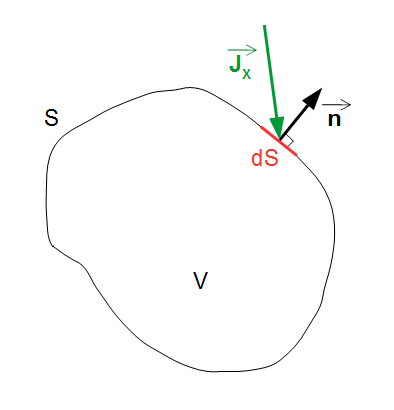
\includegraphics[scale = 0.8]{bilan.png}
		\caption{Schéma de support pour le bilan local, refaire au tableau.}
	\end{center}
\end{figure}

\subsubsection{Terme d'échange}
\`A travers dS et pendant dt, le système échange avec le milieu extérieur une quantité
\begin{equation}
	d\Phi_X dt = - \bold{J}_X\cdot\bold{n}dS,
\end{equation}
où $d\Phi_X$ est un flux de X échangé avec le milieu extérieur et $\bold{J}_X$ une densité volumique de flux. Si $\bold{J}_X$ est parallèle à la surface, il n'y a pas d'échange. S'il est perpendiculaire à la surface, l'échange est maximal, d'où le produit scalaire. \'A travers toute la surface du système, on a finalement
\begin{equation}
	\boxed{\delta X^r = - dt \oiint \bold{J}_X\cdot\bold{n}dS}.
\end{equation}

\newpage
On doit distinguer deux types de contributions dans $\bold{J}_X(\bold{r},t)$ :
\begin{itemize}
	\item la densité volumique de courant de \textbf{convection} $\bold{J}_X^{\text{CONV}}$, liée à 	un déplacement moyen de matière (déplacement global d'une particule fluide directement lié à la 	valeur locale du champ des vitesses) : 
	\begin{equation}
		\bold{J}_X^{\text{CONV}}(\bold{r},t) = n_v \bold{v},
	\end{equation}
	où $\bold{v} = \bold{v}(\bold{r},t)$ désigne le champ des vitesses du milieu continu par 			rapport au référentiel d'étude et $n_v(\bold{r},t)$ est la densité volumique de particules.
	En effet, un élément de matière dont le centre de masse traverse $d\Sigma$ pendant $dt$ à la 		vitesse $\bold{v}$ se trouve à l'instant $t$ contenu dans un cylindre de volume $\bold{v}dt			\cdot\bold{n}d\Sigma$.\\

	\item le courant de \textbf{conduction} $\bold{J}_u^{\text{COND}}$, lié au phénomène de 			diffusion, est défini comme la différence entre $\bold{J}_u$ et le courant de convection 
	$\bold{J}_u^{\text{CONV}}$ :
	\begin{equation}
		\bold{J}_u^{\text{COND}}(\bold{r},t) = \bold{J}_u - \bold{J}_u^{\text{CONV}}.
	\end{equation}
\end{itemize}
Dans toute la suite nous supposerons l'absence de convection dans le système.\\

\subsubsection{Terme de création}
On définit un taux de création locale, par unité de temps et de volume $\tau_c$. Ainsi,
\begin{equation}
	\boxed{\delta X^c = dt \iiint \tau_c d\mathcal{V}}.
\end{equation}

\subsubsection{Équation de conservation}
En réunissant toutes les expressions calculées précédemment et en simplifiant par dt :
\begin{equation}
	\iiint \frac{\partial x_v}{\partial t} d\mathcal{V} + \oiint \bold{J}_X\cdot\bold{n}dS
	= \iiint \tau_c d\mathcal{V}.
\end{equation}
En utilisant le théorème de Green-Ostrogradsky et le fait que cette équation soit vraie quelque soit $V$, on obtient
\begin{equation}
	\boxed{\frac{\partial x_v}{\partial t} + \text{div}\;\bold{J}_X = \tau_c}.
\end{equation}

\subsection{Quelques exemples de grandeurs transportées}

\subsubsection{Particules}

Il est possible d'établir une équation de conservation analogue pour toute grandeur extensive caractéristique d'un système, pourvu qu'un équilibre thermodynamique local soit défini.\\ 

La densité volumique de masse et la densité volumique particulaire du système sont définies comme
\begin{equation}
	M = \iiint \rho d\mathcal{V} \qquad\text{et}\qquad N = \iiint n_v d\mathcal{V},
\end{equation}
$M$ et $N$ étant la masse totale et le nombre total de particules contenus dans le système de volume $\mathcal{V}$. Ainsi, en l'absence de réaction chimique ou nucléaire (sinon on ajoute des termes source), l'équation de conservation du nombre de particules s'écrit
\begin{equation}
	\boxed{\frac{\partial n_v}{\partial t} + \text{div}\;\bold{J}_n = 0},
\end{equation}
où $n_V$ désigne la densité volumique de particules.\\

Si on suppose un transport purement convectif de particules, $\bold{J}_n = n_v \bold{v}$ : en multipliant par la masse des particules, on obtient l'équation de continuité de la mécanique des fluides :
\begin{equation}
	\boxed{\frac{\partial \rho_m}{\partial t} + \text{div}\;\left(\rho_m \bold{v}\right) = 0},
\end{equation}
où $\rho_m = m n_v$ est la densité volumique de masse locale.

\subsubsection{Champ électromagnétique}

Considérons le champ électromagnétique comme système. Ce problème est un peu plus exotique que les précédents, car un milieu matériel n'est pas nécessaire à l'existence d'un champ électromagnétique. On a alors l'équation suivante
\begin{equation}
	\boxed{\frac{\partial}{\partial t} \left( \frac{\epsilon_0 E^2}{2} + \frac{B^2}{2\mu_0}\right)
	+ \text{div}\;\bold{R}
	= - \bold{E}\cdot\bold{J}_q}
\end{equation}
où $\bold{R} = \bold{E}\times\bold{B}/\mu_0$ est le vecteur de Poynting (densité volumique de flux d'énergie électromagnétique) et $\bold{J}_q$ est la densité volumique de courant électrique. Cette équation est physiquement assez complexe, car elle fait intervenir l'effet Joule, un transfert d'énergie du champ électrique vers les particules chargées (milieu extérieur dans notre modèle). Le vecteur de Poynting décrit quant à lui un transport par rayonnement.

\newpage
\section{Le transport de chaleur}

On va s'intéresser au transport d'énergie sous forme de chaleur.

\subsection{Modes de transport de la chaleur}

Il existe trois grands modes de transport de la chaleur :\\
\begin{itemize}
	\item \textcolor{red}{conduction :} elle requiert un milieu matériel et naît de l'inhomogénéité 	de l'agitation thermique. Elle conduit à l'homogénéisation de l'agitation thermique par 			transfert d'énergie de proche en proche. Cette homogénéisation se fait grâce aux collisions 		dans les milieux fluides (gaz, liquides), et grâce aux vibrations du réseau cristallin (solides 	isolants électriques) ou à la circulation des électrons de conduction (solides conducteurs 			électriques chauds). De façon intuitive, on comprend qu'elle est surtout efficace sur de 			courtes distances (plusieurs fois le libre parcours moyen dans un gaz, plusieurs fois la taille 	caractéristique du réseau cristallin dans un solide isolant)\\

	\textbf{Exemples :} de l'énergie est transportée par conduction
	\begin{itemize}
 		\item lorsqu'on plaque sa main contre un fer à repasser brûlant,
		\item lorsqu'un glaçon déposé sur une surface à température ambiante fond.\\
	\end{itemize}
\end{itemize}

\begin{itemize}
	\item \textcolor{red}{convection :} elle requiert un milieu matériel fluide (liquide ou gaz) ou 	hautement déformable (manteau terrestre, métaux en  fusion). La matière voyage et transporte 		avec elle son énergie interne, qui est ainsi transportée d'un point à un autre. Elle peut 			ensuite être communiquée par simple contact avec la matière environnante, par conduction. Ces 		deux modes de transport sont souvent couplés. C'est un mode de transport efficace sur des 			distances importantes (tant que l'énergie n'est pas dissipée d'une autre manière), qui écrase 		assez vite la conduction.

	\textbf{Exemples :} de l'énergie est transportée par convection 
	\begin{itemize}
 		\item lorsqu'en approchant les mains au-dessus d'un feu, on sent de l'air chaud monter 				(convection naturelle),
		\item lorsqu'on se refroidit en utilisant un éventail (convection forcée).\\
	\end{itemize}
\end{itemize}

\begin{itemize}
	\item \textcolor{red}{rayonnement :} c'est le seul des trois modes à pouvoir fonctionner dans 		le vide absolu. Le rayonnement se propage dans le vide ou dans un milieu transparent. Un objet 		chaud émet un rayonnement électromagnétique dans tout l'espace. Ce rayonnement pourra être 			réabsorbé par un autre objet, situé beaucoup plus loin (distances astronomiques s'il n'y a pas 		d'absorption au milieu du chemin), qui verra son énergie interne augmenter.

	\textbf{Exemples :} de l'énergie est transportée par rayonnement
	\begin{itemize}
 		\item lorsqu'on ressent la chaleur d'un feu de bois à plusieurs mètres du foyer,
		\item lorsqu'on ressent la chaleur dégagée par une ampoule électrique à une distance de 1m 			(il n'y a pas de circulation d'air pour la véhiculer, et c'est trop loin de la source pour 			être de la conduction).\\
	\end{itemize}
\end{itemize}

Durant le reste de cette leçon, nous allons principalement nous intéresser à la conduction thermique, résultant d'un processus de diffusion d'énergie. On établira toutefois des analogies avec la diffusion de particules, la conduction électrique et la diffusion de quantité de mouvement, les méthodes de raisonnement et les équations qui en découlent étant très similaires.

\newpage
\subsection{Bilan d'énergie interne}

\textcolor{blue}{Soit un système au repos à l'échelle macroscopique (centre de masse immobile), mécaniquement isolé (pas de force ou champ extérieur agissant sur lui), de volume $\mathcal{V}$ constant délimité par une surface fermée $\Sigma$.} Dans toute la suite, on suppose $\delta U^c = 0$ : pas de "source" d'énergie à l'échelle mésoscopique (cela pourrait être la chaleur dégagée par des réactions chimiques ou nucléaires, par exemple). L'énergie interne du système est définie comme
\begin{equation}
	U = \iiint n_u\left(\bold{r},t\right)\;d\mathcal{V}
\end{equation}
et on trouve l'équation de conservation de l'énergie
\begin{equation}
	\displaystyle{\frac{\partial n_u}{\partial t} + \text{div}\bold{J}_u = 0}
	\label{eq:energy_conservation_local}
\end{equation}
vérifiée en tout point du système.

\subsubsection{Utilisation du Premier Principe}

Il s'agît maintenant de connecter l'équation de conservation (issue d'une modélisation de type milieu continu du problème) aux principes physiques de la thermodynamique, que l'évolution du système doit respecter. Le Premier Principe stipule que
\begin{equation}
	dU = \delta Q,
\end{equation}
en l'absence d'échange d'énergie sous forme de travail.

On a donc
\begin{equation}
	\delta U^r = \delta Q = - dt\oiint \bold{J}_u\cdot\bold{n}dS,
\end{equation}
où $\bold{J}_u$ correspond à une densité volumique de flux de chaleur.

\subsection{Loi de Fourier}

En étudiant la conduction thermique, Joseph Fourier a établi à partir de \textbf{considérations expérimentales} la loi qui porte aujourd'hui son nom. Il s'agît donc d'une \textbf{loi phénoménologique}. \textbf{En l'absence d'échanges sous forme de travail et de convection}, la densité volumique de flux d'énergie interne peut s'écrire
\begin{equation}
	\boxed{\bold{J}_u^{COND} = - \lambda \;\text{\textbf{grad}}(T)}.
	\label{eq:Fourier_law}
\end{equation}
Autrement dit, Fourier suppose que la densité volumique de flux de chaleur en tout point est proportionnelle au gradient de température local. On retrouve le \textbf{lien entre diffusion et agitation thermique non homogène} mentionné dans l'introduction. Ici, $T = T(\bold{r},t)$ désigne le champ de température, défini en tout point du système.\\

La grandeur $\lambda$ est la \textbf{conductivité thermique}, mesurée en $\text{W}.\text{m}^{-1}.\text{K}^{-1}$.

\subsubsection{Ordres de grandeur}

\textcolor{red}{Manip qualitative : déposons un glaçon identique sur deux surfaces :} l'une est faite de bois, l'autre de métal (poêle). Le glaçon déposé sur le métal fond plus vite
que celui déposé sur le bois, parce que la conductivité thermique du métal est supérieure à celle du bois. Quelques ordres de grandeur pour se donner une idée $(W.m^{-1}.K^{-1})$ :

\begin{figure}[h!]
	\begin{center}
		\begin{tabular}{|c|c|}
		\hline
		\textbf{Matériau} & $\lambda$ $(W.m^{-1}.K^{-1})$\\
		\hline
		Eau & $0.6$\\
		\hline
		Air & $24\times10^{-3}$\\
		\hline
		Cuivre & $389$\\
		\hline
		Bois et contreplaqué & $\times10^{-1}$\\
		\hline
		Béton & $1$\\
		\hline
		Verre & $1$\\
		\hline
		Acier & $\times10^{1}$\\
		\hline
		Diamant & $10^3$\\
		\hline
		\end{tabular}
	\end{center}
	\caption{Ordres de grandeur de la conductivité thermique dans différents matériaux}
\end{figure}

De façon générale
\begin{equation}
	\boxed{\text{solide métallique} > \text{solide non-métallique} 
	\geq \text{liquide} > \text{gaz}}
\end{equation}

Les bons conducteurs électriques sont assez souvent bons conducteurs de chaleur, car ce sont les mêmes porteurs qui transportent les deux quantités. La réciproque n'est pas forcément vraie (diamant, isolant électrique).

\subsubsection{Remarque 1 : introduction du Second Principe dans le modèle}
En accord avec le Second Principe, l'énergie thermique diffuse spontanément du chaud vers le froid, donc dans la direction opposée au gradient de température, d'où le signe moins dans \eqref{eq:Fourier_law}.

\subsubsection{Remarque 2 : analogies}

Les lois phénoménologiques de type Fourier, traduisant une proportionnalité entre conséquence (une densité volumique de courant) et une cause modélisée par le gradient d'une variable intensive, sont monnaie courante pour décrire, en première approximation, les phénomènes de transport.\\

Le transport de \textbf{charge électrique par conduction} est décrit localement par la \textbf{loi d'Ohm} :
\begin{equation}
	\bold{J}_e^{COND} = \sigma \bold{E}.
\end{equation}
où $\sigma$ est la conductivité électrique du milieu supposé isotrope, mesurée en Siemens par mètre(S/m). Pour les métaux, elle est supérieure à $10^6 S/m$, pour les semi-conducteurs elle est comprise entre $10^{-6}$ et $10^{4}$ (graphite) S/m. Si le champ $\bold{E}$ est d'origine purement électrostatique, alors $\bold{E} = -\textbf{grad}(V)$, où $V$ est le potentiel électrostatique.\\

Le transport de \textbf{particules par conduction}, comme dans le cas de la goutte d'encre plongée dans l'eau, est décrit localement par la \textbf{loi de Fick} :
\begin{equation}
	\bold{J}_n^{COND} = - D\;\textbf{grad}(n_v),
\end{equation}
où $D$ est le coefficient de diffusion, mesuré en $m^2s^{-1}$.\\

Enfin, supposons un fluide animé par un champ des vitesses dirigé selon $z$, inhomogène dans la direction $x$ (cisaillement). Le transport de \textbf{quantité de mouvement dans un fluide du fait de sa viscosité}, obéit localement à la relation
\begin{equation}
	\bold{J}_\bold{p}^{COND} = - \eta \left(\frac{\partial v_z}{\partial x} \right) \bold{e}_x,
\end{equation}
avec $\eta$ la viscosité dynamique, mesurée en Poiseuille (Pl). Pour l'eau, $eta = 10^{-3}$ Pa.s, pour l'air $\eta = 10^{-5}$ Pa.s, pour le miel $eta \simeq 10$ Pa.s et pour la glycérine $\eta = 1.5$ Pa.s.

\newpage

\subsubsection{Remarque 3 : Limites de validité}
Ce lien simple entre cause (un gradient de température) et conséquence (un courant) n'est pas valable dans tous les cas :
\begin{itemize}
	\item le gradient doit rester assez faible pour que la linéarité soit vérifiée;
	\item le gradient ne doit pas varier trop vite dans le temps, sinon la réponse n'est plus 				instantanée;
	\item dans un milieu anisotrope, le gradient et la densité de courant ne sont pas 						nécessairement colinéaires. La conductivité thermique est modélisée dans ce cas par un 				tenseur.
\end{itemize}

\subsection{Équation de diffusion thermique}

On combine l'équation locale de conservation de l'énergie \eqref{eq:energy_conservation_local} avec la loi de Fourier \eqref{eq:Fourier_law}:
\begin{equation}
	\frac{\partial n_u}{\partial t} + \text{div}\left(-\lambda\;\textbf{grad}(T)\right) = 0,
	\label{eq:combine_1}
\end{equation}

Définissons l'énergie interne par unité de masse, $u$, telle que, pour une particule fluide de volume $d\mathcal{V}$, de masse $dm$ et d'énergie interne $dU$ :
\begin{equation}
	n_u = \frac{dU}{d\mathcal{V}} = \frac{dU}{dm}\frac{dm}{d\mathcal{V}} = \rho_m u,
\end{equation}
où $\rho_m$ est la densité volumique de masse définie plus haut.

Supposons que \textbf{$\rho_m$ soit stationnaire} (acceptable en l'absence de convection) et \textbf{$\lambda$ soit homogène}. Dans ce cas, \eqref{eq:combine_1} devient
\begin{equation}
	\rho\frac{\partial u}{\partial t} -\lambda \left(\Delta T\right) = 0,
\end{equation}
où le symbole $\Delta$ désigne l'opérateur Laplacien.

En l'absence de convection
\begin{equation}
	du = \frac{\partial u}{\partial t} dt,\quad\text{et, d'après le Premier Principe,}\quad
	\boxed{du = c_{V} dT}.
\end{equation}
en l'absence de variation de volume. Rappelons que $c_V$ désigne la capacité calorifique massique à volume constant. Toujours sans convection,
\begin{equation}
	dT = \frac{\partial T}{\partial t}dt,
\end{equation}
d'où, en rassemblant les morceaux, l'\textbf{équation de diffusion thermique}
\begin{equation}
	\boxed{\frac{\partial T}{\partial t} = a\Delta T}.
\end{equation}

La grandeur
\begin{equation}
	\boxed{a \equiv \frac{\lambda}{\rho c_{V}}}
\end{equation}
désigne le coefficient de diffusion thermique, ou \textbf{diffusivité thermique} mesuré en $m^2s^{-1}$.

Cette équation implique une dérivée première par rapport au temps et une dérivée seconde par rapport à l'espace : ce n'est pas une équation d'onde.

\subsubsection{Remarque 1 : cas uni-dimensionnel}
En coordonnées cartésiennes : $T = T(x,t)$,
\begin{equation}
	\boxed{\frac{\partial T}{\partial t} = a\frac{\partial^2 T}{\partial x^2}}.
\end{equation}

\subsubsection{Remarque 2 : Théorème de superposition}
Cette équation différentielle est linéaire : le théorème de superposition est applicable.

\subsubsection{Remarque 3 : Irréversibilité}
L'équation n'est pas invariante par rapport à l'opération de renversement du temps $t \rightarrow -t$. C'est une manifestation de l'irréversibilité fondamentale du processus de diffusion. Les quantités transportées se déplacent spontanément dans le sens opposé au gradient qui génère le transport.

\subsubsection{Remarque 4 : Analogie avec le transport de particules}

La diffusion de particules obéit à l'équation 
\begin{equation}
	\frac{\partial n}{\partial t} = D\;\Delta n,
\end{equation}
où $D$ est le coefficient de diffusion particulaire, qui s'exprime lui aussi en $\text{m}^2/s$. Le coefficient de diffusion dépend de la nature de la particule qui diffuse et du milieu dans lequel elle diffuse. Cette équation a exactement la même forme que l'équation de diffusion thermique.

\subsubsection{Remarque 5 : Ordres de grandeurs de coefficients de diffusion}
Déterminer la valeur d'un coefficient de diffusion est une première approche pour caractériser un phénomène de transport diffusif dans un système. Voici quelques ordres de grandeurs pour :\\
\begin{itemize}
	\item le transport de chaleur
	\begin{figure}[h!]
		\begin{center}
			\begin{tabular}{|c|c|}
			\hline
			\textbf{Milieu} & a $(\text{m}^2/\text{s})$\\
			\hline
			Cuivre & $10^{-4}$\\
			\hline
			Acier & $10^{-5}$\\
			\hline
			Béton & $5\times10^{-7}$ \\
			\hline
			Eau & $10^{-7}$\\
			\hline
			Air & $2\times 10^{-5}$\\
			\hline
			\end{tabular}
		\end{center}
	\end{figure}
	
	\item le transport de matière
	\begin{figure}[h!]
		\begin{center}
			\begin{tabular}{|c|c|}
			\hline
			\textbf{Type de diffusion} & D $(\text{m}^2/\text{s})$\\
			\hline
			Molécules dans un gaz & $10^{-6}$ à $10^{-4}$\\
			\hline
			Molécules dans un liquide & $10^{-12}$ à $10^{-8}$\\
			\hline
			Atomes dans un solide & $10^{-30}$ à $10^{-16}$ \\
			\hline
			\end{tabular}
		\end{center}
	\end{figure}
\end{itemize}
\newpage
\section{Résolution de l'équation de diffusion}

\subsection{En régime stationnaire}

Reprenons l'exemple du transport de chaleur par diffusion.

\subsubsection*{Expression du champ de température}

En régime stationnaire, l'équation de diffusion de la chaleur se résume à l'équation de Laplace
\begin{equation}
	\boxed{\Delta T = 0}.
\end{equation}

D'autre part, l'équation de conservation de l'énergie implique
\begin{equation}
	\boxed{\text{div}\bold{J}_u = 0},
\end{equation}
donc une densité volumique de flux d'énergie homogène dans tout le système.\\

Pour un problème uni-dimensionnel : $T(\bold{r},t) = T(x)$ et $\bold{J}_u = J_{u}\bold{e}_x = -\lambda\;\frac{dT}{dx}$, d'où
\begin{equation}
	\frac{d^2 T}{d x^2} = 0 \qquad \Rightarrow \qquad \frac{dT}{dx} = \text{cte} = -\frac{J_u}{\lambda}
\end{equation}
d'où
\begin{equation}
	\boxed{T(x) = - \frac{J_u}{\lambda}x + \text{Cte}}
\end{equation}
avec $\text{Cte} = T(x=0)$ : les \textbf{conditions de bord} vont nous permettre de préciser la solution.

\subsubsection*{Résistance thermique}

On veut isoler une pièce à température $T_1$ de l'air extérieur, considéré comme thermostat de température $T_0$. Pour cela on interpose un mur, isolant d'épaisseur $e_1$, de surface $S$ et de conductivité thermique $\lambda_1$ entre les deux milieux. Loin du plafond et loin du sol, on peut considérer qu'il y a invariance par translation selon $y$ et $z$. Le problème est donc uni-dimensionnel. On se place en régime stationnaire. Dans le mur, le profil de température est donc donné par la solution à l'équation de diffusion la chaleur établie juste au-dessus :
\begin{equation}
	T(x) = -\frac{J_u}{\lambda_1}x + T_0.
\end{equation} 
 
On a donc 
\begin{equation}
	T(e_1) = T_1 = -\frac{J_u}{\lambda_1}e_1 + T_0 
\end{equation}

Introduisons l'intensité du flux thermique $I_u$, définie comme $I_u = J_u S$.
Ainsi, la relation qui lie $T_0 - T_1$ à $I_u$,
\begin{equation}
	T_0 - T_1 = I_u\frac{e_1}{\lambda_1 S},
\end{equation}
est \textbf{de la forme de la loi d'Ohm globale en électrocinétique}. La différence de température joue le rôle de la tension, et l'intensité du flux thermique celui de l'intensité du courant électrique. Ce n'est pas surprenant compte tenu de la similitude entre la loi de Fourier et la loi d'Ohm locale.

On peut donc définir en général une \textbf{résistance thermique}, mesurée en $K.W^{-1}$,
\begin{equation}
	R_{th} \equiv \frac{T_0 - T_1}{I_u},\quad\text{qui dans notre cas vaut}\quad
	R_{th} = \frac{e_1}{\lambda_1 S}.
\end{equation}

Lorsque cette résistance est faible, elle conduit bien la chaleur. Lorsqu'elle est forte, elle isole. Les lois de composition des résistances thermiques sont les mêmes que pour les résistances électriques :
\begin{itemize}
\item deux résistances thermiques $R_1$ et $R_2$ placées en série sont équivalentes à une résistance $R_1 + R_2$;
\item lorsque deux résistances thermiques sont associées en parallèle, ce sont les conductances thermiques $1/R_{th}$ qui s'ajoutent.
\end{itemize}

\subsubsection*{Expérience : mesure d'une conductivité électrique}

La conductivité électrique dans un métal n'est pas un phénomène de diffusion. La conduction n'est donc pas nécessairement un phénomène de diffusion. Dans un métal, l'équation de Poisson s'écrit
\begin{equation}
	\Delta V = -\frac{\rho}{\epsilon_0},
\end{equation}
avec $V$ le potentiel électrique et $\rho$ la densité volumique de charge. Ce n'est pas une équation de diffusion. Néanmoins, la densité volumique de charge est nulle en régime stationnaire, du fait de la neutralité électrique du conducteur. On retombe sur une équation de Laplace typique de la diffusion en régime stationnaire.\\ 

On peut donc établir une analogie entre conduction thermique et conduction électrique (même équation en régime stationnaire, loi phénoménologique de même forme). La solution sera du même type que celle établie pour l'équation de la chaleur : 
\begin{equation}
	V_A - V_B \equiv U = R I,
\end{equation}
entre deux bornes A et B entre lesquelles circule un courant électronique d'intensité $I$. Dans cette expression, R est la \textbf{résistance électrique} du conducteur
\begin{equation}
	R = \frac{\ell}{\sigma S}
\end{equation}
où $\ell$ désigne la longueur du conducteur et $S$ sa section.\\ 

On souhaite mesurer la conductivité électrique $\sigma$ du cuivre : pour cela on fait circuler un courant constant dans un fil de cuivre entre deux bornes séparées d'une longueur $L$ qu'on peut faire varier. On trace $U = f(L)$ et on mesure S au pied à coulisses.

\begin{equation}
	\lambda = 401\;\text{W}.\text{m}^{-1}.\text{K}^{-1} \quad
	\sigma = 59.6\times 10^{6}\;\text{S}.\text{m}^{-1}
\end{equation}

\subsubsection*{Température de contact}

On colle un second conducteur, de nature différente, au premier. On reste en régime stationnaire et on suppose que les températures $T_0$ et $T_2$ sont maintenues constantes. On a alors
\begin{equation}
	T_0 - T_c = I_u R_1
\end{equation}
et
\begin{equation}
	T_0 - T_2 = I_u\left(R_1 + R_2\right)
\end{equation}
d'où
\begin{equation}
	T_0 - T_c = \frac{R_1}{R_1 + R_2}\left(T_0 - T_2\right)
\end{equation}
On reconnaît une expression analogue au diviseur de tension.\\

En supposant des plaques de même épaisseur $e \equiv e_1 = e_2$, la température de contact $T_c$ s'écrit :
\begin{equation}
	\displaystyle{T_c = \frac{R_2T_0 + R_1 T_2}{R_1 + R_2} = \frac{\frac{e_2}{\lambda_2}T_0 + \frac{e_1}{\lambda_1}T_2}{\frac{e_1}{\lambda_1} + \frac{e_2}{\lambda_2}}}
	= T_c = \frac{T_0\lambda_1 + T_2\lambda_2}{\lambda_1 + \lambda_2}.
\end{equation}

\subsubsection*{Exemple : contact d'une main avec une plaque chauffée}
\begin{itemize}
\item Main à température $T_2 = 293$K ($\lambda_2 = 0.5$) S.I. au contact d'une plaque de cuivre à $T_1 = 373$K ($\lambda_1 = 390$ S.I.) : $T_c \simeq 373 K$.\\

\item La même main (ou ce qu'il en reste) au contact d'une plaque de bois portée à $T_1 = 373$K, comme le cuivre auparavant. On trouve $T_c \simeq 316 K$, soit 43 degrés Celsius, une température supportable.
\end{itemize}

Le cuivre conduit tellement bien la chaleur que la température est quasiment homogène dans toute la plaque. On se brûle au contact. Ce n'est pas le cas avec le bois, qui bloque la chaleur. 

\subsection{En régime non-stationnaire}

Pour résoudre l'équation de diffusion, il nous faut :
\begin{itemize}
	\item des conditions aux limites du domaine où aura lieu la diffusion,
	\item la condition initiale.\\
\end{itemize}

On s'intéresse à l'évolution d'une goutte d'encre dans un milieu. Pour simplifier le problème, on travaillera à une dimension. L'équation de diffusion de l'encre s'écrit
\begin{equation}
	\frac{\partial n_v}{\partial t} = D \frac{\partial^2 n_v}{\partial x^2}.
\end{equation}

Pour $t > 0$, on peut montrer que la solution s'écrit 
\begin{equation}
	n(x,t) = \frac{N_0}{2\sqrt{D\pi t}}\text{exp}\left(-\frac{x^2}{4Dt} \right) 
	\quad\text{avec}\quad \int_{-\infty}^{+\infty} dx n(x,t) = N_0
\end{equation}
le nombre total de particules d'encre.\\

On peut évaluer la taille de la tâche d'encre en calculant la largeur à mi-hauteur de la fonction n(x,t), L(t) :
\begin{equation}
	n\left(\frac{L}{2},t\right) = \frac{n_0(t)}{2}
\end{equation}
d'où, en utilisant l'expression de n dans les deux termes, puis en passant au logarithme
\begin{equation}
	L = 4\sqrt{\text{ln}2Dt} \propto \sqrt{Dt}.
\end{equation}

Ce comportement est caractéristique des phénomènes de diffusion et permet d'expliquer pourquoi la conduction n'est pas efficace pour transporter de l'énergie sur de grandes distances par rapport à la convection. On peut le retrouver par analyse dimensionnelle de l'équation de diffusion, en posant $\tau^*$ et $L^*$ respectivement le temps caractéristique du phénomène de diffusion et la longueur caractéristique du gradient de $n$. Par analyse dimensionnelle de l'équation de diffusion, on trouve
\begin{equation}
	L^* \sim \sqrt{a\tau^*} \propto \sqrt{\tau^*}.
\end{equation}

Si l'évolution du champ de densité est dominée par la convection, on a plutôt
\begin{equation}
	\frac{\partial n}{\partial t} + \text{div}\left(n \bold{v}\right) = 0,
\end{equation}
où on a introduit une densité volumique de courant de convection via $\bold{v}$, qui est une vitesse moyenne locale (i.e. le champ des vitesses) non-nulle. L'analyse dimensionnelle donne
\begin{equation}
	L* \sim v \tau^* \propto \tau^*.
\end{equation}
Pour transporter sur de longues distances, la convection est bien plus efficace (plus rapide). On a pu le constater en agitant le liquide dans lequel on avait versé une goutte d'encre.




\newpage
\section{Liens avec une description microscopique}

Nous avons établi les lois décrivant les phénomènes de diffusion à l'échelle macroscopique. La conductivité thermique (ainsi que les autres coefficients de diffusion mentionnés plus haut) est définie comme une constante à mesurer. Il est possible de relier cette grandeur aux propriétés microscopiques du système. 

\subsection{Marche aléatoire}

Nous allons commencer par expliquer la relation entre longueur de gradient et temps de diffusion pour un gaz parfait au repos, en l'absence de tout phénomène de convection.\\

Dans un gaz, la diffusion est liée aux collisions. Entre deux collisions, les molécules parcourent en moyenne une distance appelée libre parcours moyen (notée $\ell$) durant un temps moyen $\tau$. La trajectoire d'une molécule est donc une ligne brisée, constituée de $n$ segments de longueur $\ell$ au bout d'un temps $t$. Après chaque choc, la molécule part dans une direction totalement aléatoire, toutes les directions étant a priori équiprobables (absence de champ extérieur venant briser l'isotropie du gaz, et on regarde ce qu'il se passe loin des bords). Ce modèle est appelée "marche aléatoire" (ou marche de l'ivrogne).\\

Au bout du premier pas, $OA_1^2 = \ell^2$. Considérons une infinité de réalisations (indépendantes les unes des autres) du premier pas et moyennons (moyenne sur les réalisations) :
\begin{equation}
	\langle OA_1^2 \rangle = l^2.
\end{equation}

Supposons qu'après $(n-1)$ pas, $\langle OA_{n-1}^2 \rangle = (n-1)\ell^2$. Montrons par récurrence que $\langle OA_n^2\rangle = n\ell^2$.

Vectoriellement,
\begin{equation}
	\bold{OA_n} = \bold{OA_{n-1}} + \bold{A_{n-1}A_n},
\end{equation}
donc
\begin{equation}
	OA_n^2 = OA_{n-1}^2 + A_{n-1}A_n^2 + 2\bold{OA_{n-1}}\cdot\bold{A_{n-1}A_n}.
\end{equation}

Faisons une moyenne d'ensemble sur une infinité de marches aléatoires indépendantes partant du point O à $t = 0$ :
\begin{equation}
	\langle OA_n^2 \rangle = \langle OA_{n-1}^2\rangle + \langle A_{n-1}^2 A_n^2 \rangle + 2\langle \bold{OA_{n-1}}\cdot\bold{A_{n-1}A_n}\rangle.
\end{equation}

Le premier terme est donné par l'hypothèse. Le second terme vaut naturellement $l^2$ puisqu'il ne correspond qu'à un seul pas. Le dernier terme est nul, car la direction d'un pas est indépendante du pas le précédant. Considérant une infinité de réalisations, et car toutes les directions après un choc étant équiprobables,
\begin{equation}
	\langle \bold{OA_{n-1}}\cdot\bold{A_{n-1}A_n}\rangle = \langle \bold{OA_{n-1}}\rangle\cdot\underbrace{\langle\bold{A_{n-1}A_n}\rangle}_{=\bold{0}} = 0.
\end{equation}
On obtient donc $\langle OA_n^2\rangle = n\ell^2$. Comme l'hypothèse est vérifiée pour le premier pas, on a 
\begin{equation}
	\langle OA_n^2 \rangle = n\ell^2 = \frac{t}{\tau}\ell^2\;\forall n.
\end{equation}

On trouve une relation du type :
\begin{equation}
	\langle OA_n^2 \rangle = Dt, \quad\text{où}\quad D = \ell^2/\tau.
\end{equation}

L'écart moyen par rapport à la position initiale augmente avec la racine carrée du temps, comportement caractéristique de la diffusion. On fournit là un modèle microscopique du phénomène de diffusion.

\subsection{Modèle microscopique de diffusion thermique}

Dans un fluide, la diffusion thermique a pour origine le transport de l'énergie cinétique des particules grâce aux collisions. Il y a donc un lien entre le transport de chaleur et le transport de particules. Dans les métaux purs, conducteurs électriques, ce sont les électrons de conduction qui assurent le transport de chaleur. Dans les solides isolants, l'interprétation du phénomène est différente : ce sont les vibrations des ions du réseau cristallin autour de leur position d'équilibre qui sont responsables du transport de chaleur. 

Essayons de trouver une expression pour la conductivité thermique $\lambda$. Nous laisserons de côté le cas des solides isolants qui relève d'un cours de physique du solide de niveau plus avancé. 

Comme le transport de chaleur est lié au transport de particules, nous sommes en droit d'espérer une relation de proportionnalité entre la conductivité thermique $\lambda$ (mesurée en $W.m^{-1}.K^{-1}$) et le coefficient de diffusion particulaire $D$ (mesuré en $m^2s^{-1}$).

L'analyse dimensionnelle implique
\begin{equation}
	\text{dim}\left(\frac{\lambda}{D}\right) = \frac{(ML^2T^{-3})L^{-1}\Theta^{-1}}{L^2 T^{-1}} = (ML^2T^{-2})L^{-3}\Theta^{-1}.
\end{equation}

Les paramètres qui semblent pertinents pour décrire la diffusion thermique sont ceux figurant dans l'équation de diffusion de la chaleur, la masse volumique $\rho$ (en $kg.m^{-3}$) et la capacité thermique massique à volume constant $c_V$ (en $J.kg^{-1}.K^{-1}$). Ainsi, en réunissant toutes les briques, on trouve :
\begin{equation}
	\lambda \sim \rho c_V D.
\end{equation}

Essayons maintenant de modéliser le problème de façon quantitative, par un modèle uni-dimensionnel \ref{fig:transport_1Dmicromodel}. 

\begin{figure}[h!]
	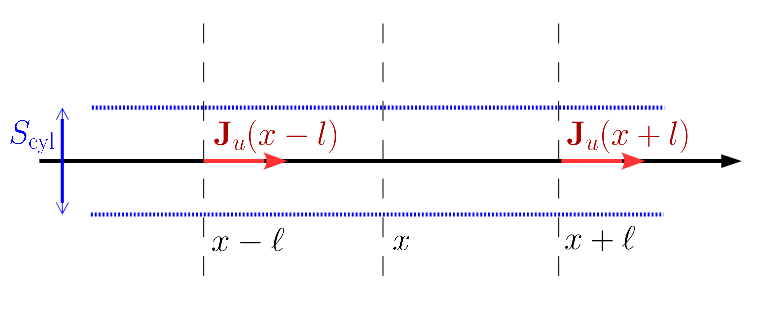
\includegraphics[scale = 0.8]{micro_cond.png}
	\caption{Modèle 1D de transport} 
	\label{fig:transport_1Dmicromodel}
\end{figure}

Soit un cylindre de section $S_{cyl}$ contenant des particules. On suppose l'isotropie de la distribution des vitesses, de sorte qu'on estime que, par unité de volume, $n_v/3$ molécules se déplacent parallèlement à l'axe $x$. La moitié de ces particules se déplacent vers la gauche ($n_v/6$), l'autre moitié ($n_v/6$) vers la droite. On note la vitesse caractéristique de l'agitation thermique des particules $v_m$.

Tout comme pour l'approche de type marche aléatoire, on suppose que les particules se déplacent avec un mouvement rectiligne uniforme entre deux chocs. On suppose enfin que les chocs ont lieu en même temps pour toutes les molécules. La durée entre deux chocs $\tau$ est donc $\tau = \ell/v_m$ (ordres de grandeur dans l'air : dans les conditions usuelles : $\ell \simeq 0, 15 \mu m $, $v_m \simeq 500 m.s^{-1}$ et $\tau \simeq 3.10^{-10} s$.\\ 

Soit $t$ l'instant du choc. Seules les molécules dont le vecteur vitesse est orienté parallèlement à la direction $x$ participeront à la diffusion. Elles vont parcourir, jusqu'à la prochaine collision, une distance $\ell$ à la vitesse $v_m$. Du fait du gradient de température, la vitesse d'agitation thermique dépend de la position des particules après un choc.

Les molécules qui vont pouvoir franchir la section de côte $x$ sont :
\begin{itemize}
\item celles qui se trouvent dans un cylindre de longueur $v_m \tau$, situées en amont de la section si leur vitesse est $+v_m \bold{e}_x$. Leur nombre est $(n_v/6) S_{cyl}v_m\tau$. En moyenne, l'énergie véhiculée par ce transport est
\begin{equation}
	\frac{n_v}{6} v_m \tau S_{cyl} \Bigg\langle m \frac{v_m^2(x-\ell)}{2} \Bigg\rangle.
\end{equation}

\item celles qui se trouvent dans le même cylindre, mais en aval de la section de côte $x$, si  leur vitesse est $-v_m \bold{e}_x$. Leur nombre est $(n_v/6) S_{cyl}v_m\tau$. En moyenne, l'énergie véhiculée s'écrit
\begin{equation}
	\frac{n_v}{6} v_m \tau S_{cyl} \Bigg\langle m \frac{v_m^2(x+\ell)}{2} \Bigg\rangle.
\end{equation}
\end{itemize}

On néglige la dépendance spatiale de la vitesse thermique pour le calcul du nombre de particules, mais on la prend en considération dans le calcul de l'énergie transportée. Ceci est bien entendu une approximation.

La quantité résultante d'énergie échangée de part et d'autre de la section de côte $x$ pendant la durée $\tau$ s'écrit
\begin{equation}
	\frac{n_v}{6}v_m \tau S_{cyl} \Bigg\langle m \frac{v_m^2(x-\ell)}{2} - m \frac{v_m^2(x+\ell)}{2} \Bigg\rangle,
\end{equation}
comptée positivement si le transport résultant va de la gauche vers la droite.
 
On va supposer que la température ne varie pas pendant la durée élémentaire $dt$, qui doit être grande devant $\tau$ mais faible devant la durée de relaxation du gradient de température. Dans ce cas, la quantité résultante d'énergie échangée pendant $dt$ est tout simplement la somme de quantités égales échangées chacune pendant la durée $\tau$ :
\begin{equation}
	\frac{n_v}{6}v_m dt S_{cyl} \Bigg\langle m \frac{v_m^2(x-\ell)}{2} - m \frac{v_m^2(x+\ell)}{2} \Bigg\rangle.
\end{equation}

On divise par $S_{cyl}dt$ pour obtenir la densité volumique de flux d'énergie au point $x$ :
\begin{equation}
	J_u = \frac{n_v}{6}v_m \Bigg\langle \frac{m}{2}v_x^2(x-\ell) - \frac{m}{2}v_x^2(x+\ell) \Bigg\rangle.
\end{equation}
Le théorème d'équipartition de l'énergie implique que $\langle mv_x^2/2 \rangle = k_B T/2$, d'où, en faisant un DL de la température à l'ordre 1,
\begin{equation}
	J_u = - \frac{\ell v_m}{2} \frac{n_v k_B}{2} \frac{\partial T}{\partial x}.
\end{equation}
Comme $n_v k_B/2$ représente la contribution d'une dimension à la capacité thermique volumique $\rho c_V$ du fluide, on trouve
\begin{equation}
	J_u = -\frac{\ell v_m}{3}\rho c_V\frac{\partial T}{\partial x}.
\end{equation}

On peut montrer avec la même approche que le coefficient de diffusion de particules $D$ vaut
\begin{equation}
	D = \frac{\ell v_m}{3},
\end{equation}
d'où
\begin{equation}
	\lambda = \rho c_V D = \frac{\ell v_m}{3}\rho c_V.
\end{equation}

\newpage
\subsubsection{Estimation du libre parcours moyen (facultatif)}

Il faut ensuite trouver une estimation du libre parcours moyen en fonction du cas considéré : 
\begin{itemize}
\item pour un gaz parfait, on peut démontrer que
\begin{equation}
	D = \frac{(RT)^{3/2}}{\sigma(T) p M^{1/2}},
\end{equation}
où $\sigma$ est la section efficace du processus de collision intervenant dans la diffusion. 
En utilisant la loi des gaz parfaits, on peut montrer que
\begin{equation}
	\lambda = \frac{C_{Vm}}{\sigma}\left(\frac{RT}{M}\right)^{1/2}
\end{equation}
où $C_{Vm}$ est la capacité calorifique molaire à volume constant. La conductivité thermique est indépendante de la pression, ce qui est bien vérifié expérimentalement.

\item pour un liquide, le libre parcours moyen est estimé comme étant la distance moyenne entre deux particules. On prend la vitesse du son dans le liquide $c_s$ comme valeur de $v_m$ et on a $\rho c_V \sim 3R/V$.
\end{itemize}

Dans un solide conducteur, on peut démontrer la loi de Wiedemann-Franz, qui établit que le rapport des conductivités thermique $\lambda$ et électrique $\gamma$ (calculée avec le modèle de Drude) est proportionnel à la température :
\begin{equation}
	\frac{\lambda}{\gamma} = \frac{3}{2}\frac{k_B}{e}^2 T.
\end{equation}
Ni la masse et ni la concentration des porteurs n'intervient dans cette expression, ce qui tend à montrer que ce sont les mêmes particules (les électrons, en l'occurence) qui sont responsables du transport des deux quantités. Cette loi illustre le fait que les bons conducteurs électriques sont aussi de bons conducteurs thermiques. La loi de Wiedemann-Franz n'est pas valable pour décrire des isolants. Un bon conducteur thermique comme le diamant n'est, par exemple, pas capable de conduire l'électricité.
 
\section{Conclusion}

\begin{itemize}
\item Un écart à l'équilibre thermodynamique provoque un transport d'une ou plusieurs grandeurs extensives : nombre de particules, quantité de mouvement, masse, charge électrique, énergie. Plusieurs modes transport sont possibles, par exemple pour la chaleur : convection, rayonnement, diffusion.\\

\item L'étude des processus de transport de la chaleur est un enjeu industriel majeur : on citera par exemple l'isolation thermique des bâtiments. La compréhension des phénomènes de transport d'énergie est également un enjeu de taille dans de nombreux domaines de la recherche en physique : mécanique des fluides, météorologie, plasmas de fusion pour ne citer qu'eux.\\

\item Lorsque l'échelle mésoscopique n'existe pas et/ou que les gradients sont trop forts, les lois phénoménologiques type Fourier ne s'appliquent plus. Il est alors souvent nécessaire de faire appel à une approche cinétique, c'est à dire microscopique.
\end{itemize}

\section*{Annexes}

\end{document}